\cotefile{34}
\scanpage{196}
\mspage{II.44}
% archive sheet number: 195
% lines 1--12
\deleted{\unsure{Et|Si} $X$ est en car $p>0$, alors $X$ est \unsure{gros}.}

Si $X$ est en car $p>0$ $(p=0)$, alors $X\to\operatorname{Spec}\mathbb{F}_p=S$ induit \deleted{\unsure{un}} \unsure{quasi-isom.} $\pi_1(X,\unsure{\xi|\eta})\unsure{-|\to}\pi_1(S,\xi)\simeq\widehat{\mathbb{Z}}$, donc le $\pi_1(X,\xi)^{\unsure{\mathrm{alg}}}\to(\widehat{\mathbb{Z}}^{\mathrm{alg}})$ est un quasi-\deleted{\unsure{isomorphisme}}\inserted{\unsure{épim.}}, et $\widehat{\mathbb{Z}}^{\mathrm{alg}}$ (comme on sait \unsure{aussitôt}) est de dim infinie. Si $X$ est en car $p>0$, alors \unsure{faisant} $S=\operatorname{Spec}\mathbb{Z}[1/\unsure{\ell|l}]$, \deleted{\unsure{on} $\Pi=\pi_1(X,\xi)\to\pi_1(S,$} en raisonnant de $=$, on montre que $\pi_1(S)$ a \deleted{\unsure{un quotient}} comme plus gd \unsure{quotient} abélien $\mathbb{Z}_\ell^*$, qui est quasi-isomorphe à $\mathbb{Z}_\ell$, or $\mathbb{Z}_\ell^{\mathrm{alg}}$ est aussi de dim. infinie ....

% lines 13--21
6.16. Revenons aux conditions générales de 6.13. L'intérêt de la considération de \deleted{\unsure{\(\Pi\)}} $\Pi=\pi_1^{\mathrm{arith}}(X,\xi)$ tient au fait que tous les faisceaux $\ell$-adiques \unsure{constants tordus} qui \unsure{rencontrons|se rencontrent} pratiquement sont de nature arithmétique; \unsure{i.e.|ou.} proviennent déjà d'un tel faisceau sur un $X_\lambda$, \unsure{est unique modulo isom.|et unique modulo isom.} \unsure{?}, sur un $X_\mu$, avec $\mu\gg\lambda$. \deleted{En d'autres termes,} De $=$ pour les \unsure{hom} de faisceaux $\ell$-adiques. En d'autres termes,
\scanpage{197}
\mspage{II.45}
% archive sheet number: 196
% lines 1--6
Il y a lieu de travailler dans la catégorie $\underset{\lambda}{\varinjlim}$ (faisceaux \unsure{cts} tordus sur $X_\lambda$), qui précisément s'explicite en termes de représentations \uline{linéaires} \inserted{$\unsure{\ell|l}$-adiques} du pro groupe $\Pi$, ou en termes de $\Pi^{\unsure{\mathrm{alg}|\mathrm{an}}}$, ou de rep. alg. de $\Pi^{\unsure{\mathrm{alg}|\mathrm{an}}}$.

% lines 7--13
\uline{Exemple 1} Soit $f:Y\unsure{-|\to}X$ un morphisme propre et lisse, on prend les $R^i f_*(\deleted{\unsure{\mathbb{Z}}}\mathbb{Q}_{\ell Y})$, \unsure{on|ou} \deleted{\unsure{en déduit|on déduit}} les $R^i f_*(\deleted{\unsure{\mathbb{Z}}}\mathbb{Q}_{\ell Y})$ si on veut une représentation de $\unsure{\widetilde G|\widetilde C},\unsure{\widetilde{\mathfrak g}|\widetilde g}$. De $=$, les hom entre $R^i f_*$ définis par des $X$-morphismes $Y\unsure{-|\to}Y'$, ou $[$\deleted{\unsure{si}} $X$ est intègre normal) par des \deleted{classes de} correspondances \inserted{algébriques} sur les fibres \unsure{génériques|géométriques}.

% lines 14--20
\uline{Exemple} $^2$ (\unsure{ess\textsuperscript{t} identique}). $T_\ell(A)$, où $A$ est un schéma abélien sur $X$, \deleted{$\unsure{=T_\ell(A)\otimes_{\mathbb{Z}_\ell}\mathbb{Q}_\ell}$} Noter que $\underline{\operatorname{Hom}}(T_\ell(A),\deleted{\unsure{\mathbb{Q}}}\mathbb{Z}_\ell)\simeq R^1 f_*(\mathbb{Z}_{\ell A})$, donc $T_\ell(A)$ et $R^1 f_*(\mathbb{Z}_{\ell A})$ se déterminent mutuellement. \deleted{\illegible{2}} Si on veut en déduire une représentation de $\widetilde{\mathfrak g}=\operatorname{Lie}(\pi_1^{\mathrm{arith}}(X;\unsure{\xi|\eta}))$, il faut \unsure{tensoriel|tensoriser} d'abord par $\mathbb{Q}_\ell$.
\scanpage{198}
\mspage{II.46}
% archive sheet number: 197
% lines 1--5, with insertion in upper margin
Bien entendu, les exemples 1, 2 \inserted{de rep. de $\Pi^{\unsure{\mathrm{an}}}$ ou $\Pi^{\unsure{\mathrm{alg}}}$} ont un caractère \uline{fonctoriel} pour $X$, resp $A$, variable. En particulier, dans le cas d'une $A$, on trouve un hom d'anneaux (injectif),
\[
\operatorname{End}(A)\otimes_{\mathbb{Z}}\mathbb{Q}_{\unsure{\ell|l}}\hookrightarrow\operatorname{End}_{\Pi}\bigl(\underbrace{T_\ell(A(\unsure{\xi|\eta}))\otimes_{\mathbb{Z}_\ell}\mathbb{Q}_\ell}_{E}\bigr).
\tag*{(\unsure{6.15.1|6.16.1})}
\]

% lines 6--17
\uline{Remarque 6.16.} Une des conséquences des \uline{conjectures de Tate}, (qui montre le rôle essentiel des représentations \unsure{obtenues|linéaires|retenues} des \unsure{gr|gpes|gps} fondamentaux \deleted{\unsure{géom.}} \unsure{arithmétiques|arithmetiques}) est que l'hom précédent est bijectif \deleted{\unsure{Ce}} lorsque $X$ est normal intègre. Pour cette question, on se ramène d'ailleurs aussitôt au cas où $X$ est le spectre d'un corps \uline{algébrique clos}. Cela montre à quel point ($=$ dans un cas soi-disant ``géométrique'') l'opération de $\Pi$ est loin d'être triviale. [C'est prouvé par Tate si $X$ est le spectre d'un corps fini, \deleted{\unsure{et}} ou \deleted{\unsure{partant dans le}} \inserted{de façon équivalente,} si c'est le spectre de la clôture algébrique d'un corps fini .... ].

% lines 18--22
\uline{Remarque} 6.17. On s'est rendu compte que $\Pi$ lui-$=$, ou $G=\Pi^{\mathrm{an}}$, $\unsure{\widetilde G|\overline G}=\Pi^{\mathrm{alg}}$, $\unsure{\mathfrak g^\circ|\mathfrak g^\bullet}$, $\unsure{\widetilde{\mathfrak g}|\overline{\mathfrak g}}$, sont démesurément grands et ils échappent pratiquement à notre contrôle. Leur rôle est surtout théorique, i.e. leurs représentations $\ell$-adiques
\scanpage{199}
\mspage{II.47}
% archive sheet number: 198
% lines 1--7
Dans chaque pb géométrique particulier, \unsure{on n'a guère qu'à} considérer les représentations (analytiques ou algébriques) se \unsure{factorisant|factorisent} par un gpe \deleted{quotient} $\unsure{G|C}_\alpha$ resp. $\widetilde G_\alpha$ fixé du syst. projectif, dont on peut espérer que c'est l'image dans un $\underline{\operatorname{Aut}}_{\mathbb{Q}_{\unsure{\ell|l}}}(E)$ d'un gpe $\pi_1(X_\lambda,\unsure{\xi|\eta}_\lambda)$, resp. son enveloppe algébrique.

% lines 8--14
Notons que \deleted{\unsure{pour tout le}} dans (6.15.1) l'opération de $\Pi$ sur $E$ définit un gpe algébrique $\widetilde G_E\subset\underline{\operatorname{Aut}}_{\mathbb{Q}_\ell}(E)$, enveloppe algébrique d'un gpe analytique $G_E$ \deleted{\unsure{provenant}} \inserted{image} d'un $\pi_1(X_\lambda,\xi)$, et que le deuxième \unsure{membre} de (6.15.1), peut aussi s'écrire, \unsure{même|mais} formellement, $\operatorname{End}_{G_E}(E)=\operatorname{End}_{\widetilde G_E}(E)$.

% lines 15--19
Si $\pi_1(X,\xi)$ (\uline{non} arith) $=1$ (p. ex $X$ le spectre d'un corps sep clos) alors ce deuxième membre est aussi $\operatorname{End}_{\unsure{\mathfrak g|g}_E}(E)=\operatorname{End}_{\widetilde{\mathfrak g}_E}(E)$, où $\mathfrak g_E=\operatorname{Lie}(G_E)\subset\operatorname{End}(E)$ et $\widetilde{\mathfrak g}_E$ est l'enveloppe algébrique de $\mathfrak g_E$ ....
\scanpage{200}
% archive sheet number: 199
% title block, upper right
SGA 7 \unsure{II|III|IV} \uuline{appendice}

Application des conjectures standart sur les cycles algébriques.
\scanpage{201}
% archive sheet number: 200
1) \uline{Cohomologie des diviseurs à croisements normaux.}

\[
\begin{aligned}
\underset{\text{propre}}{Y}=\bigcup_\alpha Y_\alpha\qquad &Y_\alpha\ \text{projectif et lisse,}\\
&Y_{\alpha_0}\cap\cdots\cap Y_{\alpha_p}\ \text{est lisse.}
\end{aligned}
\]
\[
H^{\unsure{*|\bullet}}(Y,\mathbb{Q}_{\unsure{\ell|l}})\Longleftarrow E_2^{pq}=H^p(\sigma\mapsto H^q(Y_\sigma,\mathbb{Q}_\ell)),\qquad
Y_{\alpha_0\cdots\alpha_p}=Y_{\alpha_0}\cap\cdots\cap Y_{\alpha_p}
\]
\deleted{\unsure{Proposition}} \deleted{\unsure{Théorème}}

$E_2^{pq}$ est de \uline{poids} $q$ donc $d_r^{pq}$ est nulle pour tout $r$.
% slanted
\margin{\uline{NB} de plus (\unsure{via} conjectures standard) les dimensions des $E_2^{pq}$ sont indépendantes de $\ell$.}
$H^i(Y,\mathbb{Q}_\ell)$ \unsure{se dévisse} en les $E_2^{p,q}$ $(p+q=i)$, de poids $0,1,\ldots,i$.

2) Cohomologie des \deleted{variétés} \inserted{schémas} quasi-projectifs lisses non propres.

$X=X'-Y$, $X'$ projectif et lisse, $Y$ diviseur à croisements normaux, tels que les comp. irréduc. $Y_i$ soient lisses.
\[
\begin{aligned}
H^{i-1}(X',\mathbb{Q}_\ell)\to\underset{\text{poids }\leq i-1}{H^{i-1}(Y,\mathbb{Q}_\ell)}\to H^i_{\deleted{\unsure{c}}!}(X,\mathbb{Q}_\ell)\to\underset{\text{poids }i}{H^i(X',\mathbb{Q}_\ell)}\to\underset{\text{poids }\leq i}{H^i(Y,\mathbb{Q}_\ell)}\to H^{i+1}_!(X,\mathbb{Q}_\ell)\to\cdots
\end{aligned}
\tag*{\textcircled{1}}
\]

On trouve que
\[
\text{a) }\deleted{\text{l'image}}\ \operatorname{Im}(H^{i-1}(Y,\mathbb{Q}_\ell)\inserted{\to H^i_!(X,\mathbb{Q}_\ell)})=\operatorname{Ker}(H^i_!(X,\mathbb{Q}_\ell)\unsure{-|\to}H^i(X',\mathbb{Q}_\ell))
\]
\uline{ne dépend pas} de la résolution choisie : c'est le morceau de poids $\leq i-1$ de $H^i_!(X,\mathbb{Q}_\ell)$.

\deleted{De plus, le \unsure{Ker et le Coker}}

\unsure{Le|Les} Ker et Coker de $H^i(X',\mathbb{Q}_\ell)\overset{\varphi^i}{\unsure{-|\to}}H^i(Y,\mathbb{Q}_\ell)$, à isom. can. près, est aussi indépendant de la résolution choisie. \deleted{\unsure{Ce dernier se dévisse en un}} \inserted{Considérons la filtration de} $H^i(Y,\mathbb{Q}_\ell)$ provenant de la suite spectrale étudiée dans 1), correspond. à un \unsure{déviss. gr} en $E_2^{pq}=H^p(\sigma\mapsto H^q(Y_\sigma,\mathbb{Q}_\ell))$ $(p+q=i)$. L'hom.
% formula crowded against the right and lower edges
\[
H^i(Y,\mathbb{Q}_\ell)\unsure{-|\to}E_2^{0,i}=H^0(\sigma\mapsto H^i(Y_\sigma,\mathbb{Q}_\ell))=\operatorname{Ker}(\deleted{\unsure{\bigoplus}}\unsure{\prod_\alpha}H^i(Y_\alpha,\mathbb{Q}_\ell)\inserted{\to\cdots})
\]
\scanpage{202}
\mspage{-2.12-}
% archive sheet number: 201
The ``only if'' in (ii) is proven in the same way: assume $(0)\handwritten{\unsure{\in|\epsilon}}$ closure $O(x^*)$. As a first step, we obtain a $K$-valued point $\handwritten{\phi}$ of $G$ such that $(0)$ is the specialization of $\handwritten{\psi_{{\unsure{x|\chi}}^*}\circ\phi}$ when $t\handwritten{\longrightarrow}0$. We decompose $\handwritten{\phi}$ exactly as before, and obtain $(*)\handwritten{'}$. But now the term on the left hand side of $(*)\handwritten{'}$ is actually in $t\cdot R$ since $\handwritten{\sigma}^{*}\handwritten{\bigl(}(\handwritten{\psi}_1 b_2)^{-1},\handwritten{\psi_{x^*}\circ\phi\bigr)}$ actually specializes to $(0)$ when $t\handwritten{\longrightarrow}0$. Therefore, instead of (A), we obtain:
\[
X_i\handwritten{\bigl\{}\handwritten{\sigma}^{*}(b_2^{-1}\handwritten{\psi}_2,\ x^*)\handwritten{\bigr\}}\handwritten{\in}t^{-r_{\handwritten{i}}+1}\cdot R\ .
\tag*{($\overset{\handwritten{\sim}}{A}$)}
\]

(B) is the same as before, hence combining $(\overset{\handwritten{\sim}}{A})$ and (B) it follows that $r_i>0$ whenever $X_i(x^*)\handwritten{\neq}0$. Therefore, $\handwritten{\mu}(x,b_2^{-1}\handwritten{\lambda}\ b_2)<0$ and (ii) is proven. \uline{QED}

A second application of Iwahori's theorem is:

\uline{Proposition} \uline{2.4}: Let a reductive algebraic group $G$ over $k$ act via $\handwritten{\sigma}$ on an algebraic scheme $X$ over $k$. Then the action of $G$ is proper if and only if for every non-trivial 1-PS $\handwritten{\lambda}:\handwritten{\mathbb{G}}_m\handwritten{\longrightarrow}G$, the induced action of $\handwritten{\mathbb{G}}_m$ on $X$ is proper.
% vertical marginal rule beside Proposition 2.4
\figure{\begin{tikzpicture}\draw (0,0)--(0,1.8);\end{tikzpicture}}

\uline{Proof}: The only if is clear. To prove the if, suppose the action of $G$ is not proper, i.e. $\handwritten{\Psi}:G\times X\handwritten{\longrightarrow}X\times X$ is not proper. Then, by the valuative criterion for properness, there are $K$-valued points $\handwritten{\phi}$ and $\handwritten{\xi}$ of $G$ and $X$ respectively such that $\handwritten{\Psi(\phi\times\xi)}$ is an $R$-valued point of $X\times X$, but $\handwritten{\phi\times\xi}$ is not an $R$-valued point of $G\times X$. In other words, $\handwritten{\xi}$ and $\handwritten{\sigma(\phi,\xi)}$ are $R$-valued points of $X$, but $\handwritten{\phi}$ is not an $R$-valued point of $G$. By Iwahori's theorem, we can write
\scanpage{203}
% archive sheet number: 202
induit un hom injectif $\operatorname{Im}\varphi^i\unsure{-|\to}E_2^{0,i}$, i.e. $\operatorname{Im}\varphi^i\cap\operatorname{Filt}^1(H^i(Y,\mathbb{Q}_{\unsure{\ell|l}}))=0$, de sorte que \deleted{$\operatorname{Coker}\unsure{\varphi}$} la filtration quotient sur $\operatorname{Coker}\varphi^i$ a comme facteurs \deleted{$\unsure{E_2^{0,i}}$}
\[
\begin{aligned}
\operatorname{Coker}(H^i(X)\unsure{-|\to}E_2^{0,i})&=\text{défaut d'exactitude de}\\
H^i(X)\unsure{-|\to}\prod H^i(Y_\alpha)&\longrightarrow H^i(Y_{\alpha\beta})^{\unsure{\ell}},
\end{aligned}
\]
les $E_2^{p,q}$ $(p\geq1,\ p+q=i)=\deleted{\unsure{\prod_{\alpha_0\cdots\alpha_p}H^p(Y)}}H^p(\sigma\mapsto H^q(Y_\sigma))$. Cette filtration est également indépendante de la résolution choisie des singularités, et correspond à la filtration de $H^{i+1}_!(X)$ par poids décroissants (à partir des poids $i$).
% slanted
\margin{de plus, si conj. standard, les dimensions des divers morceaux de ces filtrations \unsure{(par poids)} sur $H^i_!(X_{\unsure{\mathrm{ét}|\mathrm{et}}},\mathbb{Q}_\ell)$ \unsure{sont} indépendantes de $\ell$ !}

\textcircled{b} Par dualité, on peut considérer aussi
\[
\cdots\longrightarrow H_Y^i(X')\longrightarrow H^i(X')\unsure{-|\to}H^i(X)\longrightarrow\ ,
\]
on a d'autre part
\[
H_Y^{\unsure{n|*|\bullet}}(X)\Longleftarrow E_2^{pq}=H^p(Y,\underline H_Y^q(\mathbb{Q}_{\ell X'})),
\]
\deleted{\unsure{Or, d'autre part}}
\[
\underline H_Y^q(\mathbb{Q}_\ell)=0\ \text{si }q<2,\quad\text{et}\quad
\underline H_Y^q(\mathbb{Q}_\ell)=\mathop{\bigwedge}^{q-1}\left(\coprod_\alpha\mathbb{Q}_{\ell Y_\alpha}(-1)\right)=\deleted{\unsure{\sum}}\coprod_{\alpha_1<\cdots<\alpha_{q-1}}\mathbb{Q}_{\ell Y_{\alpha_1\cdots\alpha_{q-1}}}(-1)
\]
donc
\[
E_2^{pq}=\begin{cases}
0&\text{si }q<2\\
\displaystyle\coprod_{\alpha_1<\cdots<\alpha_{q-1}}H^p(Y_{\alpha_1\unsure{,|\cdots}\alpha_{q-1}})(-(q-1))&\text{si }q\geq2
\end{cases}
\]
donc $E_2^{pq}$ est de poids $p+2q-2$ donc on \deleted{\unsure{ne peut}} aura \deleted{$d_r=0\ \text{si}$}
\[
d_r=0\quad\text{si }r\geq3.
\]
\scanpage{204}
\mspage{-2.3-}
% archive sheet number: 203
ii) for fixed $x$ and $\handwritten{\lambda}$, $\handwritten{\mu}^{L}(x,\handwritten{\lambda})$ defines a homomorphism from $\operatorname{Pic}^{\handwritten{G}}(X)$ to $\handwritten{\mathbb{Z}}$ as $L$ varies.

iii) If $f:X\handwritten{\longrightarrow}Y$ is a $G$-linear morphism of schemes on which $G$ acts, $L\handwritten{\unsure{\in|\epsilon}}\operatorname{Pic}^{\handwritten{G}}(Y)$ and $x\handwritten{\in}X_{\handwritten{k}}$, then
\[
\handwritten{\mu}^{f*L}(x,\handwritten{\lambda})=\handwritten{\mu}^{L}(fx,\handwritten{\lambda}).
\]

iv) If $\handwritten{\sigma(\lambda(\alpha)},x)\handwritten{\longrightarrow}y$ as $\handwritten{\alpha\longrightarrow}0$, then $\handwritten{\mu}^{L}(x,\handwritten{\lambda})=\handwritten{\mu}^{L}(y,\handwritten{\lambda})$.

(Proofs Immediate).

The theorem which we shall ultimately prove is:

\uline{Theorem} \uline{2.1}: Let a \uline{reductive group} $G$ act on a scheme $X$, proper over $k$. Let $L\handwritten{\in}\operatorname{Pic}^{\handwritten{G}}(X)$, and assume $L$ is \uline{ample}. Then if $x\handwritten{\in}X_{\handwritten{k}}$:
% The underlines beneath "reductive group" and "ample" are handwritten and wavy.
\[
\begin{aligned}
x\handwritten{\in}X^{ss}(L)&\handwritten{\Longleftrightarrow}\handwritten{\mu}^{L}(x,\handwritten{\lambda})\handwritten{\geq}0\quad\text{for all 1-PS's }\handwritten{\lambda}\ ,\\
x\handwritten{\in}X^{s}_{(0)}(L)&\handwritten{\Longleftrightarrow}\handwritten{\mu}^{L}(x,\handwritten{\lambda})>0\quad\text{for all 1-PS's }\handwritten{\lambda}\ .
\end{aligned}
\]

There are two approaches to the proof of this theorem. Either we choose a $G$-linear immersion $X\handwritten{\subset\mathbb{P}_{n-1}}$, and reduce to the case $X=\handwritten{\mathbb{P}_{n-1}}$ by Theorem \figure{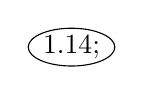
\begin{tikzpicture}[baseline=(a.base)]\node[inner sep=2pt] (a) {1.14;};\draw (a.center) ellipse[x radius=.55cm,y radius=.24cm];\end{tikzpicture}} or we can put $Y$ equal to the normalization of the closure of $\unsure{O|0}(x)$, and via the canonical $\handwritten{\pi}:Y\handwritten{\longrightarrow}X$, reduce to the case where $O(x)$ is dense in $X$ by Theorem \figure{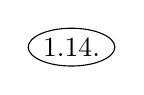
\begin{tikzpicture}[baseline=(a.base)]\node[inner sep=2pt] (a) {1.14.};\draw (a.center) ellipse[x radius=.55cm,y radius=.24cm];\end{tikzpicture}} We shall follow the former which is more down to earth. Therefore \uline{we may assume} $X=\handwritten{\mathbb{P}_{n-1}}$. Now let
% The two ovals and the underline beneath "we may assume" are handwritten.
% margin note written slanted, beside the first reference to Theorem 1.14
\margin{\handwritten{\unsure{why|w}??\\1.19\ \uline{\unsure{2|?}}}}
% right margin: pencil strokes beside "reduce to" and "follow", then an upward arrow and question mark
\figure{\begin{tikzpicture}[x=1cm,y=1cm]
\draw (0,2.2)--(.2,2.15)--(.34,1.97) (.15,2.07)--(.31,2.18);
\draw (0,1.7)--(.4,1.65) (.1,1.72)--(.06,1.52);
\draw (.1,1.2)--(.4,1.15) (.24,1.18)--(.23,.98);
\draw[->] (.23,0)--(.23,.65);
\node at (.8,.65) {\handwritten{?}};
\end{tikzpicture}}
\[
\begin{aligned}
V&=H^{\unsure{0|o}}(\handwritten{\mathbb{P}_{n-1}},\underline{o}(1))\\
\handwritten{\mathbb{A}}^{n}&=\handwritten{\mathbb{V}}(V):\text{ the affine cone over }\handwritten{\mathbb{P}_{n-1}}\ .
\end{aligned}
\]
There is a natural projection from $\handwritten{\mathbb{A}}^{n}-(0)$ to $\handwritten{\mathbb{P}_{n-1}}$. We shall say
\scanpage{205}
% archive sheet number: 204
\deleted{Il faut \unsure{donc} \unsure{prendre} $E_3^{pq}$}

Il faut \unsure{croire|voir} que $E_2^{p*}\longrightarrow$ \inserted{(\unsure{un. autre twist|un autre twist|ou autres twists})} le \deleted{\unsure{complexe des}} complexe dual de \deleted{$\unsure{E_2^{**}(Y)|E_2^{**}}$} $\sigma\mapsto H^p(Y_\sigma)$ \inserted{de \textcircled{a}}, \unsure{compte} \unsure{tenu} de la dualité de Poincaré, de sorte que \deleted{\unsure{var. de|via} $\unsure{Y_\sigma}$} ${}^{b}E_3^{**}$ est dual de ${}^{(a)}E_2^{**}$ à twist près.

\textcircled{c} Autre présentation \inserted{de $H^{\unsure{*|\bullet}}(X,\mathbb{Q}_{\unsure{\ell|l}})$} : suite spectrale de Leray de $\unsure{g|j}:X\hookrightarrow X'$; \unsure{=}
\[
H^*(X)\Longleftarrow E_2^{pq}=H^p(X',R^q g_*(\mathbb{Q}_\ell))
\]
Or
\[
\begin{aligned}
R^q g_*(\mathbb{Q}_\ell)&\simeq\mathop{\bigwedge}^{q}\coprod_\alpha\mathbb{Q}_\ell(-1)_{Y_\alpha}\\
&\simeq\coprod_{\alpha_1<\cdots<\alpha_q}\mathbb{Q}_{\ell Y_{\alpha_1\cdots\alpha_q}}(-q).
\end{aligned}
\]
Donc
\[
\left\{\begin{aligned}
E_2^{pq}&=\coprod_{\alpha_1<\cdots<\alpha_q}H^p(Y_{\alpha_1\cdots\alpha_q})(-q)\qquad\text{si }q\geq1\\
E_2^{p0}&=H^p(X')\deleted{\unsure{\mathbb{Q}_\ell}}
\end{aligned}\right.
\]
qui est \uline{de poids} $p+2q$. \uline{Donc on trouve} \deleted{\illegible{3}}
\[
\underline{d_r=0\quad\text{si }r\geq3},
\]
et il faut calculer encore $E_3^{pq}$, \deleted{\unsure{comme}} i.e. les
\diagram{\begin{tikzcd}[ampersand replacement=\&,column sep=small,row sep=large]
\&E_2^{pq}\arrow[r]\arrow[dl,equal]\&E_2^{p+2,q-1}\arrow[dr,equal]\&\\
\displaystyle\coprod_{\alpha_1<\cdots<\alpha_q}H^p(\tikz[baseline=(yl.base)]{\node[inner sep=0pt] (yl) {$Y_{\alpha_1\cdots\alpha_q}$};\node[anchor=east] (dl) at (-.55,.8) {\uline{dim $\unsure{n-1-q}$}};\draw (dl.east) to[out=0,in=90] (yl.north);})(-q)\arrow[rrr]\arrow[d,dash,"{\text{dual}}"']\&\&\&\displaystyle\coprod_{\alpha_1<\cdots<\alpha_{q-1}}H^{p+2}(\tikz[baseline=(yr.base)]{\node[inner sep=0pt] (yr) {$Y_{\alpha_1\cdots\alpha_{\unsure{q-3|q-1}}}$};\node[anchor=west] (dr) at (.55,.8) {dim $n-q$};\draw (dr.west) to[out=180,in=90] (yr.north);})(-(q-1))\arrow[d,dash,"{\text{dual}}"]\\
H^{\unsure{2n-2-p-2q|2n-2-p+2q}}(Y_{\alpha_1\cdots\alpha_q})(n-1)\&\&\&H^{2n-2q-p-2}(Y_{\alpha_1\cdots\alpha_{q-1}})(n-1)
\end{tikzcd}}
% Dimension notes have pencil leaders to the respective Y terms; the lower "dual" lines have no arrowheads.
\margin{si $q\geq2$\\i.e. $q-1\geq1$}
\figure{\begin{tikzpicture}\draw (0,0)--(0,3);\end{tikzpicture}}
\scanpage{206}
\mspage{-2.5-}
% archive sheet number: 205
1.2, as $G$ is reductive, there must be some invariant function $F\handwritten{'}$ on $\handwritten{\mathbb{A}}^n$ such that $F\handwritten{'}=0$ on $Z_2$, and $F\handwritten{'}=1$ on $Z_1$. Suppose we write:
\[
F\handwritten{'}=F_{k_1}+F_{k_2}+\cdots+F_{k_{\handwritten{\unsure{\ell|l}}}}
\]
where each $F_{k_i}$ is homogeneous of degree $k_i$. Then each $k_i$ is positive, i.e. each $F_{k_i}$ is $0$ on $Z_2$. Moreover \uline{some} $F_{k_i}$ is not zero at $x^*$. Let $F$ be that $F_{k_i}$.

By definition, $x$ is properly stable if and only if its stabilizer is finite, and for one (and hence all) $s\handwritten{\unsure{\in|\epsilon}}H^{\unsure{0|o}}(\handwritten{\mathbb{P}_{n-1}},\underline{o}_{\handwritten{\mathbb{P}}}(k))$ as above, $\unsure{O|0}(x)$ is closed in $[\handwritten{\mathbb{P}_{n-1}}]_s$ (cf. amplification \deleted{1.9}\inserted{\handwritten{1.11}}). That is to say,
% 1.11 is written in the left margin opposite the cancelled reference.
\[
\handwritten{\psi'_x}:G\handwritten{\longrightarrow}[\handwritten{\mathbb{P}_{n-1}}]_s
\]
is proper. But let $s$ correspond, as above, to the invariant homogeneous function $F$ on $\handwritten{\mathbb{A}}^n$. Then, for some non-zero $\handwritten{\alpha\in}k$, $O(x^*)$ is contained in the closed subscheme $Z_{\handwritten{\alpha}}$ of $\handwritten{\mathbb{A}}^n$ defined by $F=\handwritten{\alpha}$. Therefore
\[
\handwritten{\psi_{x^*}}:G\handwritten{\longrightarrow\mathbb{A}}^n
\]
is proper if and only if:
\[
\handwritten{\psi'_{x^*}}:G\handwritten{\longrightarrow}Z_{\handwritten{\alpha}}
\]
is proper. But let the projection from $\handwritten{\mathbb{A}}^n-(0)$ to $\handwritten{\mathbb{P}_{n-1}}$ define the morphism $\handwritten{\pi}:Z_{\handwritten{\alpha}}\handwritten{\longrightarrow}[\handwritten{\mathbb{P}_{n-1}}]$. Then, in fact: $\handwritten{\pi}(Z_{\handwritten{\alpha}})\handwritten{\subset}[\handwritten{\mathbb{P}_{n-1}}]_s$, and if $\handwritten{\pi'}$ denotes $\handwritten{\pi}$ with image taken as $[\handwritten{P_{n-1}}]_s$, then $\handwritten{\pi'}$ is
\scanpage{207}
% archive sheet number: 206
\textcircled{3}
\diagram{\begin{tikzcd}[ampersand replacement=\&,column sep=large,row sep=large]
X\arrow[d,"{f\ (\text{propre})}"']\arrow[r,phantom,"{\supset}" description,"{\unsure{g|j}}"']\&U\\
S\&\eta\ \deleted{\unsure{hens|gén}}\arrow[l,hook]\arrow[u,"{f_U}"']
\end{tikzcd}}
$X$ régulier, $U=X-\deleted{\unsure{X}}Y$, $Y=\bigcup Y_\alpha\supset X_0$
\[
\left\{\begin{aligned}
Y_\alpha&\quad\text{div. réguliers}\\
Y&\quad\text{div. à croisements normaux.}
\end{aligned}\right.
\]
\margin{\unsure{en} $Y$}
\margin{$X_0$.}
[\uline{NB} faire pour simplifier $Y=X_0$, $U=X_\eta$]
\[
H^{\unsure{*|\bullet}}(U)\Longleftarrow E_2^{pq}=H^p(X_0,R^q g_*(\mathbb{Q}_{\unsure{\ell|l}X})\vert_{X_0})
\]
\[
R^q g_*(\mathbb{Q}_{\ell X})\simeq\mathop{\bigwedge}^{q}\coprod_\alpha(\mathbb{Q}_\ell(-1)_{Y_\alpha})\simeq\coprod_{\alpha_1<\cdots<\alpha_q}\mathbb{Q}_{\ell Y_{\alpha_1\cdots\alpha_q}}(-q)
\]
donc \deleted{\illegible{1}}
\[
\left\{\begin{aligned}
E_2^{p,q}&=\deleted{\unsure{H^p}}\coprod_{\alpha_1<\cdots<\alpha_q}H^p(\deleted{\unsure{X_0}}(Y_{\alpha_1\cdots\alpha_q})_0)(-q)\qquad\text{si }q\geq1\\
E_2^{p0}&=H^p(X_0)\deleted{\unsure{\mathbb{Q}_\ell}}\quad\text{de poids }\leq\deleted{\unsure{q}}p=i\ \deleted{\text{\unsure{au plus}}}
\end{aligned}\right.
\]
\margin{de poids $p+2q=i+q$}
\[
E_r^{pq}\unsure{-|\longrightarrow}E_r^{p+r,q-r+1}
\]
a) $q-r+1\neq0$\quad poids $p+2q$ et $p+r+2(q-r+1)$\quad nulle si $r\neq2$

b) $q-r+1=0$ \deleted{\unsure{po.} $p+2q$} poids $p+2q$ et $\leq p+r$ il faut pour que $d_r^{pq}\neq0$ que l'on ait $p+2q\leq p+r$ i.e. $r\geq2q$; comme $r=q+1$, ceci s'écrit $q+1\geq2q$, i.e. $q\leq1$ donc $r\leq2$.

Donc $\underline{d_r=0}$ si $r\unsure{\geq|\gg}3$.

\deleted{En \unsure{diminuant|dimension}}

$H^i$ filtration \unsure{dont} les termes, en croissant, sont
\[
\begin{aligned}
E_2^{i0}&\quad\text{de poids }\deleted{\unsure{\leq}}i\\
E_2^{i-1,1}&\quad\text{de poids }i+1\\
E_2^{i-2,2}&\quad\text{---}\quad i+2\\[1em]
E_2^{0i}&\quad\text{---}\quad2i
\end{aligned}
\]
\margin{(lui-= muni d'une filtration \unsure{canonique} qui \unsure{correspond} aux \unsure{différents} poids\ldots)}
\scanpage{208}
\mspage{-2.11-}
% archive sheet number: 207
Therefore, since $\handwritten{\sigma}^*$ is a group action:
\[
\handwritten{\sigma}^*\handwritten{\bigl(}(\handwritten{\psi}_1\cdot b_2)^{-1},\handwritten{\psi_{{\unsure{x|\chi}}^*}\circ\phi}\handwritten{\bigr)}=\handwritten{\sigma}^*\handwritten{\bigl[}(b_2^{-1}\cdot\handwritten{\langle\lambda\rangle}\cdot b_2),\handwritten{\sigma}^*(b_2^{-1}\cdot\handwritten{\psi}_2,x^*)\handwritten{\bigr]}.
\tag*{(*)}
\]
But $(\handwritten{\psi}_1\cdot b_2)^{-1}$ is an $R$-valued point of $G$, and $\handwritten{\psi_{x^*}\circ\phi}$ is an $R$-valued point of $\handwritten{\mathbb{A}}^n$, therefore the term on the left is an $R$-valued point of $\handwritten{\mathbb{A}}^n$.

Now, if $f$ is a $\operatorname{Spec}(A)$-valued point of $\handwritten{\mathbb{A}}^n$, for some ring $A$, let us denote by $X_i(f)$ the element of $A$ which is its $i^{\mathrm{th}}$ coordinate. Then, recalling the definition of $\handwritten{\langle\lambda\rangle}$, and that $b_2^{-1}\cdot\handwritten{\lambda}\cdot b_2$ is diagonalized, equation (*) reads, in coordinates:
\[
X_i\handwritten{\bigl\{}\handwritten{\sigma}^*\handwritten{\bigl(}(\handwritten{\psi}_1 b_2)^{-1},\handwritten{\psi_{x^*}\circ\phi}\handwritten{\bigr)\bigr\}}=t^{\handwritten{\unsure{r|n}_i}}\cdot X_i\handwritten{\bigl\{}\handwritten{\sigma}^*(b_2^{-1}\cdot\handwritten{\psi}_2,x^*)\handwritten{\bigr\}}
\tag*{(*)$\handwritten{'}$}
\]
and, in particular:
\[
X_i\handwritten{\bigl\{}\handwritten{\sigma}^*(b_2^{-1}\cdot\handwritten{\psi}_2,x^*)\handwritten{\bigr\}}\handwritten{\unsure{\in|\epsilon}}t^{\handwritten{-r_i}}\cdot R.
\tag*{(A)}
\]
But $b_2^{-1}\handwritten{\psi}_2$ is an $R$-valued point of $G$, whose specialization, when $t\handwritten{\longrightarrow}0$, is the identity $e\handwritten{\in}G$; therefore $\handwritten{\sigma}^*(b_2^{-1}\handwritten{\psi}_2,x^*)$ is an $R$-valued point of $\handwritten{\mathbb{A}}^n$ whose specialization, when $t\handwritten{\longrightarrow}0$, is $x^*$; therefore
\[
X_i\handwritten{\bigl\{}\handwritten{\sigma}^*(b_2^{-1}\handwritten{\psi}_2,x^*)\handwritten{\bigr\}}=X_i(x^*)+t(Z_i)
\tag*{(B)}
\]
for some $Z_i\handwritten{\in}R$.

Combining (A) and (B), it follows that $r_i\handwritten{\geq}0$, whenever $X_i(x^*)\handwritten{\neq}0$. Therefore, $\handwritten{\mu}(x,b_2^{-1}\cdot\handwritten{\lambda}\cdot b_2)\handwritten{\leq}0$ and (i) is proven, by Proposition 2.3.
\scanpage{209}
% archive sheet number: 208
\deleted{Les \unsure{d}}
% margin note written slanted
\margin{\unsure{compatibilité} à vérifier\ldots}
\unsure{Modulo} identification des $d_2$ par morphismes canoniques (de nature ``motivique'') on trouve que la dimension des $E_\infty^{pq}$ est indépendante de $\unsure{\ell|l}$. De plus, les \deleted{valeurs propres} pol. car. de Frobenius \inserted{inverse} opérant sont à coeff. entiers entiers indépendants de $\ell$.

Utilisons la suite exacte
\[
\unsure{\bullet|0}\longrightarrow H^{i-1}(X_{\bar\eta})_I\longrightarrow H^i(\unsure{X_\eta|X_{\bar\eta}})\unsure{-|\longrightarrow}H^i(X_{\bar\eta})^I\unsure{-|\longrightarrow}0
\tag*{(\unsure{6|a})}
\]
Nous \deleted{\unsure{aurons}} \inserted{obtenons} alors des informations sur $H^{\unsure{*|\bullet}}(X_{\bar\eta})^I$ et $H^*(X_{\bar\eta})_I$, savoir

a) \unsure{leurs dimensions} indépendantes de $\ell$ $(\neq p)$

b) Les pol. car. de frobenius inverse opérant sur eux sont à coeff. entiers indépendants de $\ell$, et leurs val. propres \unsure{sont|ont} de val. absolues ${\unsure{q|1}}^{i/2}$ dans $H^i(X_{\bar\eta})^I$ et $H^i(X_{\bar\eta})_I$.

\deleted{Il suffit de le prouver pour $i\leq n$, car si c'est \unsure{vrai pour $i$, c'est} vrai pour $2n-i$ par dualité.}

On procède par récurrence sur $i$. Pour $i=0$, on a $H^0(X_\eta)\simeq H^0(X_{\bar\eta})^I$, on gagne. Pour $i>0$, \unsure{on a} \deleted{$\unsure{H^{i-1}(X_{\bar\eta})|H^i(X_{\bar\eta})}$} \unsure{utilise|utilisé} \unsure{(6)|(a)}, \deleted{\unsure{par}} et l'hyp. de récurrence.
\scanpage{210}
\mspage{-2.10-}
% archive sheet number: 209
(i) $\handwritten{\psi_{{\unsure{x|\chi}}^*}}$ is not proper if and only if for some non-trivial 1-PS $\handwritten{\lambda}$ of $G$, $\handwritten{\sigma}^*(\handwritten{\lambda(\alpha)},x^*)$ has a specialization when $\handwritten{\alpha\longrightarrow}0$.

(ii) $(0)$ is in the closure of $\unsure{O|0}(x^*)$ if and only if for some 1-PS $\handwritten{\lambda}$ of $G$, $\handwritten{\sigma}^*(\handwritten{\lambda(\alpha)},x^*)$ specializes to $(0)$ when $\handwritten{\alpha\longrightarrow}0$.

\uline{Proof}: The two ``if'' statements are obvious. Next consider the ``only if'' in (i): assume $\handwritten{\psi_{x^*}}$ is not proper. Then by the valuative criterion for properness (EGA 2, \S7), \unsure{there-is|there is} a $K$-valued point $\handwritten{\phi}:\operatorname{Spec}(K)\handwritten{\longrightarrow}G$ such that $\handwritten{\phi}$ is not induced by an $R$-valued point of $G$, but such that $\handwritten{\psi_{x^*}\circ\phi}$ is an $R$-valued point of $\handwritten{\mathbb{A}}^n$. By Iwahori's theorem, then, we know that $\handwritten{\phi}$ has the form:
\[
\handwritten{\phi}=\handwritten{\psi}_1\cdot\handwritten{\langle\lambda\rangle}\cdot\handwritten{\psi}_2
\]
for some 1-PS $\handwritten{\lambda}$ of $G$, and for $\handwritten{\psi}_1,\handwritten{\psi}_2\handwritten{\unsure{\in|\epsilon}}G(R)$. Moreover, $\handwritten{\lambda}$ is non-trivial since $\handwritten{\phi}$ is not itself an $R$-valued point of $G$. Let $b_i\handwritten{\in}G_k$ be $k$-valued point $\handwritten{\unsure{\varpi|\overline{\omega}}}(\handwritten{\psi}_i)$ obtained from $\handwritten{\psi}_i$ when $t$ specializes to $0$. By choosing suitable coordinates in $\handwritten{\mathbb{A}}^n$, we may assume that the action of $b_2^{-1}\cdot\handwritten{\lambda}\cdot b_2$ on $\handwritten{\mathbb{A}}^n$ is diagonalized. Suppose $b_2^{-1}\cdot\handwritten{\lambda(\alpha)}\cdot b_2$ acts via the matrix $(\handwritten{\alpha}^{\handwritten{\unsure{r|n}_i}}\cdot\handwritten{\delta}_{ij})$, for $\handwritten{\alpha\in}(\handwritten{\mathbb{G}}_m)_k$. Now
\[
\begin{aligned}
\handwritten{\psi_{x^*}\circ\phi}&=\handwritten{\sigma}^*(\handwritten{\phi},x^*)\\
&=\handwritten{\sigma}^*\handwritten{\bigl(}(\handwritten{\psi}_1\cdot b_2)\cdot(b_2^{-1}\cdot\handwritten{\langle\lambda\rangle}\cdot b_2)\cdot(b_2^{-1}\cdot\handwritten{\psi}_2),x^*\handwritten{\bigr)}
\end{aligned}
\]
(Here $k$-valued points of $G$ and of $\handwritten{\mathbb{A}}^n$ are identified with the $K$-valued points obtained by the base extension $K\handwritten{\supset}k$).
